\documentclass[12pt,a4paper]{article}

% packages
  \usepackage{a4wide}
  \usepackage{tikz}

  \tikzset{st/.style = {circle, thick, minimum size=5.0mm, inner sep=0pt, draw},
           we/.style = {circle, thick, minimum size=2.0mm, inner sep=0pt, draw}}

\pagestyle{empty}

\title{Graph Algorithms and Complexity Theory - Coursework 1}
\author{Oskar Mampe}
\date{Semester 1 Session 2019--2020}

\begin{document}

\maketitle

\thispagestyle{empty}

We compute a maximum flow in this network and find a minimum cut as follows.
The left column shows the actual flow and the right column shows the residual
network with residual capacities and an augmenting path indicated by bold edges.

\begin{center}
  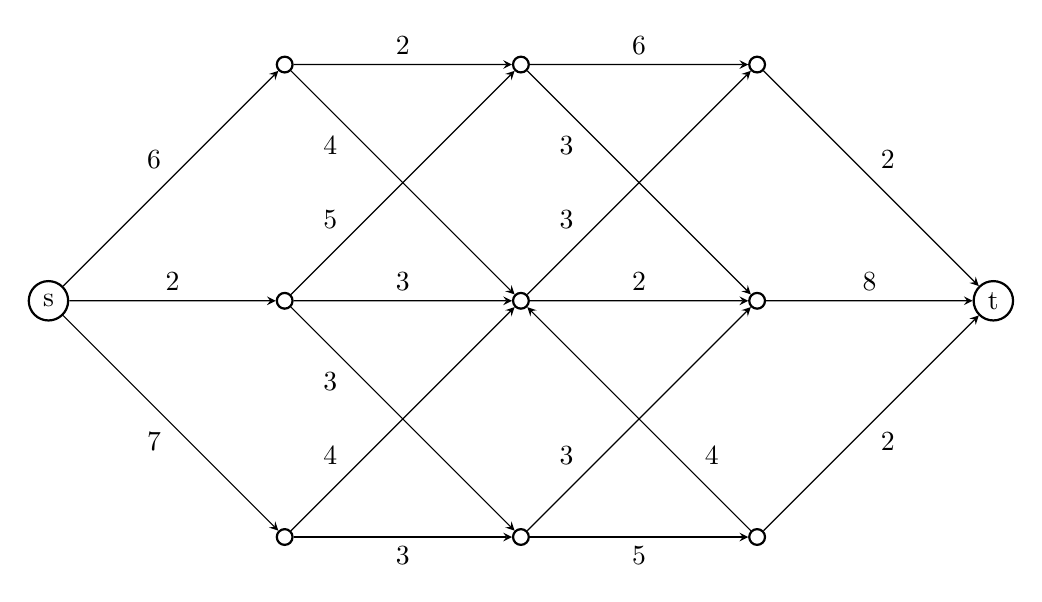
\begin{tikzpicture}[scale=1.5, >=stealth]
    \node[st] (s) at (0,2) {s};
    \node[we] (a) at (2,0) {}; \node[we] (b) at (2,2) {}; \node[we] (c) at (2,4) {}; 
    \node[we] (d) at (4,0) {}; \node[we] (e) at (4,2) {}; \node[we] (f) at (4,4) {}; 
    \node[we] (g) at (6,0) {}; \node[we] (h) at (6,2) {}; \node[we] (i) at (6,4) {}; 
    \node[st] (t) at (8,2) {t};
    \draw[->] (s) to[edge label'=7, pos=.50] (a);
    \draw[->] (s) to[edge label =2, pos=.50] (b);
    \draw[->] (s) to[edge label =6, pos=.50] (c);
    \draw[->] (a) to[edge label'=3, pos=.50] (d);
    \draw[->] (b) to[edge label =3, pos=.50] (e);
    \draw[->] (c) to[edge label =2, pos=.50] (f);
    \draw[->] (a) to[edge label =4, pos=.25] (e);
    \draw[->] (b) to[edge label =5, pos=.25] (f);
    \draw[->] (c) to[edge label'=4, pos=.25] (e);
    \draw[->] (b) to[edge label'=3, pos=.25] (d);
    \draw[->] (d) to[edge label'=5, pos=.50] (g);
    \draw[->] (e) to[edge label =2, pos=.50] (h);
    \draw[->] (f) to[edge label =6, pos=.50] (i);
    \draw[->] (d) to[edge label =3, pos=.25] (h);
    \draw[->] (e) to[edge label =3, pos=.25] (i);
    \draw[->] (f) to[edge label'=3, pos=.25] (h);
    \draw[<-] (e) to[edge label =4, pos=.75] (g);
    \draw[->] (g) to[edge label'=2, pos=.50] (t);
    \draw[->] (h) to[edge label =8, pos=.50] (t);
    \draw[->] (i) to[edge label =2, pos=.50] (t);    
  \end{tikzpicture}
    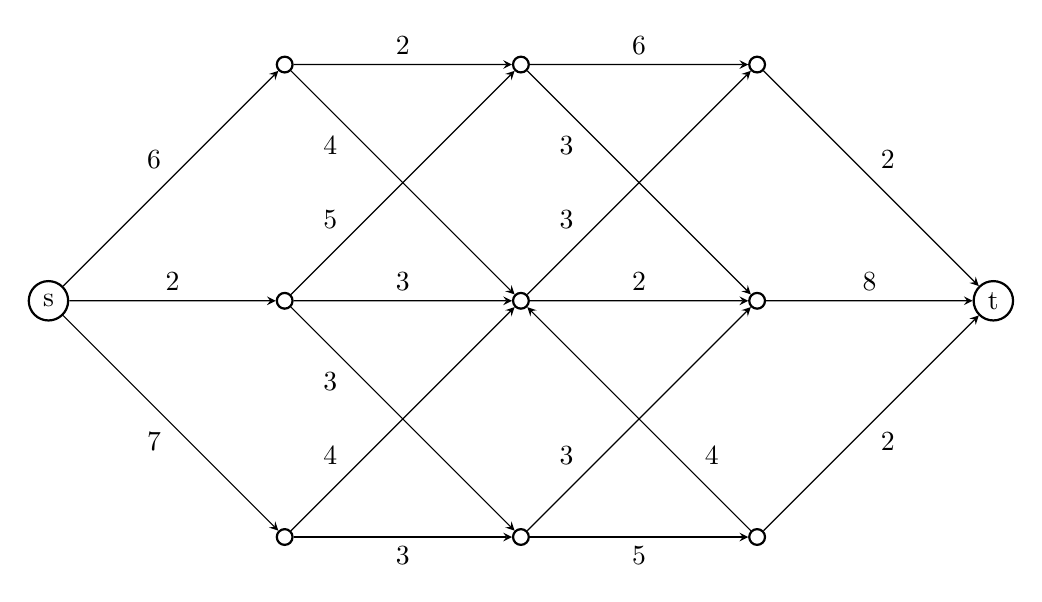
\begin{tikzpicture}[scale=1.5, >=stealth]
    \node[st] (s) at (0,2) {s};
    \node[we] (a) at (2,0) {}; \node[we] (b) at (2,2) {}; \node[we] (c) at (2,4) {}; 
    \node[we] (d) at (4,0) {}; \node[we] (e) at (4,2) {}; \node[we] (f) at (4,4) {}; 
    \node[we] (g) at (6,0) {}; \node[we] (h) at (6,2) {}; \node[we] (i) at (6,4) {}; 
    \node[st] (t) at (8,2) {t};
    \draw[->] (s) to[edge label'=7, pos=.50] (a);
    \draw[->] (s) to[edge label =2, pos=.50] (b);
    \draw[->] (s) to[edge label =6, pos=.50] (c);
    \draw[->] (a) to[edge label'=3, pos=.50] (d);
    \draw[->] (b) to[edge label =3, pos=.50] (e);
    \draw[->] (c) to[edge label =2, pos=.50] (f);
    \draw[->] (a) to[edge label =4, pos=.25] (e);
    \draw[->] (b) to[edge label =5, pos=.25] (f);
    \draw[->] (c) to[edge label'=4, pos=.25] (e);
    \draw[->] (b) to[edge label'=3, pos=.25] (d);
    \draw[->] (d) to[edge label'=5, pos=.50] (g);
    \draw[->] (e) to[edge label =2, pos=.50] (h);
    \draw[->] (f) to[edge label =6, pos=.50] (i);
    \draw[->] (d) to[edge label =3, pos=.25] (h);
    \draw[->] (e) to[edge label =3, pos=.25] (i);
    \draw[->] (f) to[edge label'=3, pos=.25] (h);
    \draw[<-] (e) to[edge label =4, pos=.75] (g);
    \draw[->] (g) to[edge label'=2, pos=.50] (t);
    \draw[->] (h) to[edge label =8, pos=.50] (t);
    \draw[->] (i) to[edge label =2, pos=.50] (t);    
  \end{tikzpicture}

\end{center}

\vspace{\fill}

The last flow has value 12. A cut $(A,B)$ of this capacity is defined
by square white vertices in $A$ and round black vertices in $B$. 
Therefore the flow is maximum and the cut $(A,B)$ is a minimum cut.
The edges across the cut $(A,B)$ are indicated by dashed lines.

\end{document}
